%
% File for Section 8.2
%
\section{Εμπιστευτικότητα -- Ακεραιότητα -- Δια\-θε\-σι\-μό\-τη\-τα -- Αυθεντικότητα -- Εγκυρότητα}

Τα βασικά προβλήματα που πρέπει να επιλύσει κάποιος κατά την ανάλυση και το σχεδιασμό του επιπέδου ασφαλείας που θέλει να πετύχει είναι τέσσερα:

\begin{itemize}

\item \textbf{Εμπιστευτικότητα (confidentaliaty):} Αποτροπή της πρόσβασης σε ιδιωτικές πληροφορίες από άτομα που δεν έχουν εξουσιοδότηση.

Για παράδειγμα, όταν κάνουμε μια ηλεκτρονική παραγγελία μέσω Διαδικτύου θέλουμε να εξασφαλίσουμε ότι ο αριθμός της πιστωτικής μας κάρτας δεν θα είναι ορατός παρά μόνο από το σύστημα  που θα τελέσει τη συναλλαγή. 

\item \textbf{Αυθεντικοποίηση (authentication) ή πιστοποίηση ταυτότητας:} Η εξασφάλιση ότι η πληροφορία προέρχεται πραγματικότητα από αυτόν που νομίζουμε (ή που ισχυρίζεται) ότι τη μετέδωσε.

Για παράδειγμα, να μπορούμε να διασφαλίσουμε ότι το άτομο που έστειλε τον αριθμό της πιστωτικής κάρτας είναι πράγματι ο κάτοχος της.  Ή όταν κάποιος εισέρχεται σε ένα υπολογιστικό σύστημα ότι πράγματι είναι το πρόσωπο στο οποίο ανήκει ο αντίστοιχος λογαριασμός χρήστη.

\item \textbf{Ακεραιότητα (integrity):} είναι η διασφάλιση ότι οι πληροφορίες δεν έχουν αλλοιωθεί και όλες οι αλλαγές που έχουν γίνει σε αυτές προέρχονται από εξουσιοδοτημένα άτομα.

Για παράδειγμα, αν κάποιος τρίτος μπορούσε να υποκλέψει τη συναλλαγή πληρωμής μιας ηλεκτρονικής αγοράς, θα μπορούσε να κατευθύνει το χρηματικό ποσό στο δικό του λογαριασμό. Μια τέτοια αλλοίωση σημαίνει απώλεια ακεραιότητας των δεδομένων.

Όταν αναφερόμαστε σε πληροφορίες, \emph{εξουσιοδοτημένα άτομα} είναι προφανώς ο αρχικός δημιουργός της πληροφορίας και τα άτομα στα οποία αυτός έχει δώσει τα αντίστοιχα δικαιώματα πρόσβασης (μερικούς ή πλήρης). 

\item \textbf{Μη Άρνηση Ταυτότητας (non-repudiation):} Η μη-αποποίηση των ευθυνών εκ των υστέρων χρηστών που συμμετείχαν σε μια ηλεκτρονική επικοινωνία.

Ουσιαστικά αυτό σημαίνει ότι μπορούμε να επιρρίψουμε με σιγουριά ευθύνες σε χρήστες για κινήσεις ή παραλήψεις που έκαναν κατά τη διάρκεια μιας επικοινωνίας αφού μπορούμε να είμαστε σίγουροι για τους συμμετέχοντες και το ρόλο του καθενός. Είναι σημαντικό οι συμμετέχοντες σε μια επικοινωνία που χειρίζεται εμπιστευτικές πληροφορίες, να μη μπορούν να αρνηθούν την εμπλοκή τους. 

Ο συνδυασμός της Αυθεντικότητας (πιστοποίηση ταυτότητας) και της Ακεραιότητας (μη αλλοίωσης) των δεδομένων είναι γνωστός ως \emph{Εγκυρότητα (val\-i\-di\-ty)} των πληροφοριών. 

Σε περιπτώσεις που είναι απαραίτητη η αδιάλειπτη παροχής πρόσβασης σε πληροφορίες από εξουσιοδοτημένους χρήστες, ορίζεται και η έννοια της \emph{διαθεσιμότητας} των πληροφοριών. Για παράδειγμα αν μια εταιρεία που διαθέτει λογαριασμούς ηλεκτρονικού ταχυδρομείου δεν μπορεί να εξυπηρετήσει τους εξουσιοδοτημένους χρήστες της λόγω επίθεσης στο δίκτυο της, αυτό αποτελεί απώλεια διαθεσιμότητας.
\end{itemize}

\begin{inthebox}
\textbf{Ασφάλεια των πληροφοριών} είναι η επίτευξη του σχεδιαζόμενου επιπέδου διαθεσιμότητας, ακεραιότητας και εμπιστευτικότητας των πληροφοριών.\\
\end{inthebox}

Για την εξασφάλιση της εμπιστευτικότητας των πληροφοριών, η πιο συχνά χρησιμοποιούμενη τεχνική είναι η κρυπτογράφηση: Σκοπός της κρυπτογράφησης είναι η μετατροπή ενός αρχικού μηνύματος με τρόπο τέτοιο ώστε να μη μπορεί να διαβαστεί από οποιονδήποτε εκτός από τον τελικό παραλήπτη. Προφανώς ο παραλήπτης θα χρησιμοποιήσει την αντίστροφη τεχνική (αποκρυπτογράφηση) για να αποκαλύψει την αρχική πληροφορία. Όσο αφορά την ασφάλεια σε μια μετάδοση δεδομένων, θεωρούμε ότι πάντα υπάρχει κάποιος που προσπαθεί να υποκλέψει τις πληροφορίες που μεταδίδουμε και ότι έχει πιθανότητες να το πετύχει.

\begin{figure}[!ht]
 \centering
 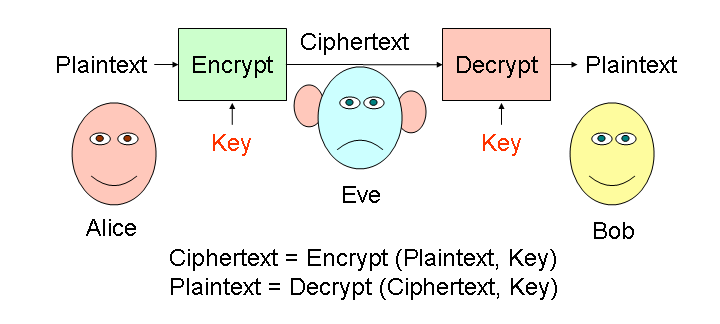
\includegraphics[width=0.95\textwidth]{images/chapter8/8-1}
 \caption {\textsl{Κρυπτογραφημένη Επικοινωνία}}
 \label{8-1}
\end{figure}

\begin{itemize}
\item \textbf{Κρυπτογράφηση} είναι η εφαρμογή μιας τεχνικής, συνήθως ένος μαθηματικού αλγόριθμου, μετατροπής της πληροφορίας από μορφή απλού κειμένου σε μορφή μη-αναγνωρίσιμη ώστε να μην είναι προσβάσιμη κατά τη μεταφορά της από μη εξουσιοδοτημένα άτομα
\item \textbf{Αποκρυπτογράφηση:} είναι μια τεχνική αντίστροφη της κρυπτογράφησης που εφαρμόζεται μόνο από εξουσιοδοτημένα άτομα σε κρυπτογραφημένη πληροφορία ώστε να επανέλθει στην αρχική μορφή απλού κειμένου
\item \textbf{Κρυπτογράφημα (ή κρυπτόγραμμα, ciphertext)} είναι η μη-αναγνωρίσιμη μορφή που προκύπτει όταν υποστεί κρυπτογράφηση το αρχικό απλό κείμενο
\item \textbf{Κλειδί (key)} είναι ένας κωδικός από ψηφιακά δεδομένα (μια σειρά από bytes ή ένα αρχείο π.χ.) το οποίο χρησιμοποιείται από τον αλγόριθμο κρυπτογράφησης / αποκρυπτογράφησης για την αντίστοιχη διαδικασία
\end{itemize}

\begin{figure}[!ht]
 \centering
 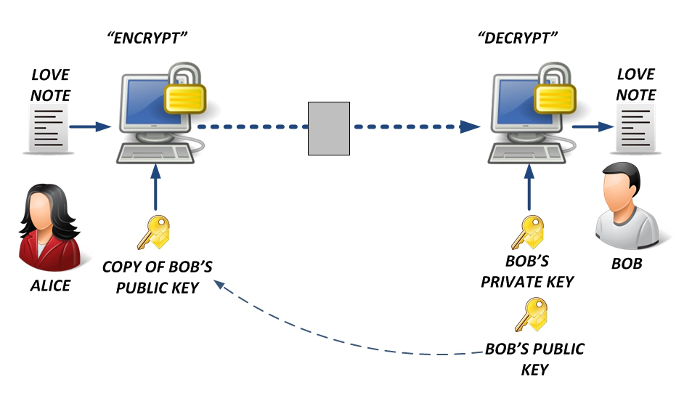
\includegraphics[width=0.95\textwidth]{images/chapter8/8-2}
 \caption {\textsl{Κρυπτογράφηση Δημόσιου Κλειδιού}}
 \label{8-2}
\end{figure}

Υπάρχουν δυο βασικά είδη κρυπτογράφησης: στην \emph{συμμετρική} κρυπτογράφηση χρησιμοποιείται το ίδιο κλειδί τόσο για την κρυπτογράφηση όσο και για την αποκρυπτογράφηση. Στην περίπτωση αυτή το κλειδί ονομάζεται και \emph{μυστικό κλειδί (secret key)} καθώς όποιος το έχει μπορεί προφανώς να αποκρυπτογραφήσει το μήνυμα. Είναι σημαντικό σε αυτή την περίπτωση το κλειδί να μη διαρρεύσει και πρέπει επίσης να βρεθεί ασφαλής τρόπος για να δοθεί σε όλα τα ενδιαφερόμενα μέρη. 

Αντίθετα στην \emph{κρυπτογράφηση με δημόσιο κλειδί} (σχήμα \ref{8-2}) ή μη-συμμετρική κρυπτογράφηση, κάθε χρήστης διαθέτει δύο κλειδιά: ένα \emph{δημόσιο κλειδί (public key)} και ένα \emph{ιδιωτικό κλειδί (private key)}. Η ιδέα εδώ είναι ότι όλοι ανταλλάσσουν τα δημόσια κλειδιά τους ενώ κρατάνε τα ιδιωτικά ως μυστικά. Στη κρυπτογράφηση δημόσιου κλειδιού, ότι κλειδώνει με το δημόσιο κλειδί ξεκλειδώνει μόνο με το αντίστοιχο ιδιωτικό (τα κλειδιά δημιουργούνται ως ζεύγη). Έτσι αν ο χρήστης Α θέλει να στείλει ένα ιδιωτικό μήνυμα στον Β, χρησιμοποιεί το δημόσιο κλειδί του Β για να το κρυπτογραφήσει. Το μήνυμα έπειτα μπορεί να αποκρυπτογραφηθεί μόνο από τον Β χρησιμοποιώντας το ιδιωτικό κλειδί του.